\documentclass[12pt]{article}
\usepackage{times}
\pagestyle{empty}
\parindent 0px
\renewcommand{\familydefault}{\sfdefault}
\usepackage{geometry}
 \geometry{
 a4paper,
 total={170mm,257mm},
 left=20mm,
 top=20mm,
 }
\title{CS5691: Assignment 1}
\author{Akshat Meena (CS19B052)}
\date{}
\usepackage{graphicx}
\graphicspath{ {../plots/} }


\begin{document}
\maketitle

\begin{enumerate}
	\begin{large}
	\item \textbf{Motivation}
	\end{large}\\
		Many images have unnecessary details stored in them which are indistinguishable to the naked eye. Using EVD/SVD we can get the those eigenvalues/singular values that contain those details. So we can construct a new image by removing those values and lower the size of the image with very less improvisation. In this experiment we will look into the effect of EVD/SVD on the quality of an grayscale image.\\
	\begin{large}
	\item \textbf{EVD/SVD}\\
	\end{large}
EVD - Eigenvalue decomposition is the factorization of a matrix into a canonical form, whereby the matrix is represented in terms of its eigenvalues and eigenvectors.\\
The decomposition can be derived from the fundamental property of eigenvectors: 
$$Av = \lambda v$$
Reconstruction of the matrix from EVD:
$$A = P.D.P^{-1}$$
Where D is the diagonal matrix of all the eigenvalues and P is the column matrix of eigenvectors.\\

SVD - the singular value decomposition (SVD) is a factorization of a real or complex matrix. It generalizes the eigendecomposition of a square normal matrix with an orthonormal eigenbasis to any $m x n$ matrix.\\
Reconstruction of the matrix from SVD:
$$A = U.\Sigma .V$$
Where $\Sigma$ is the diagonal matrix for singular values. U is the column matrix of eigenvectors of $A.A^T$and V is the transpose of column matrix of eigenvectors of $A^T.A$\\
	\begin{large}
	\item \textbf{Experimental Results}
	\end{large}\\
	
		Below are the results for some values of k
		\begin{itemize}
		\item k = 25\\
			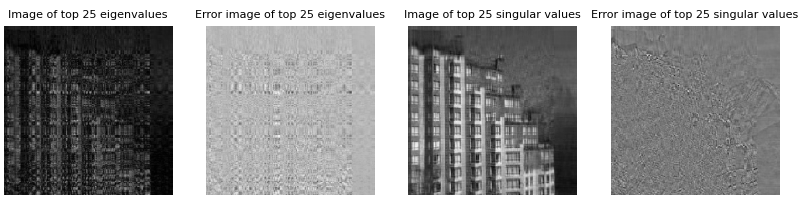
\includegraphics[scale= 0.8]{25}
		\item k = 50\\
			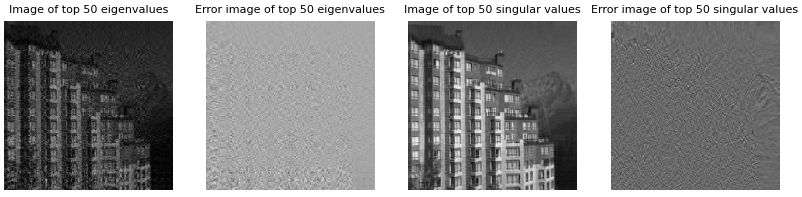
\includegraphics[scale= 0.8]{50}
		\item k = 200\\
			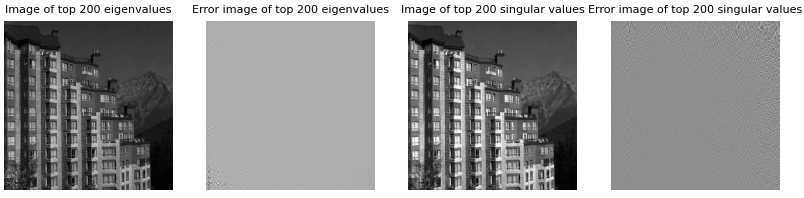
\includegraphics[scale= 0.8]{200}
		\end{itemize}

		Below are the reconstruction error vs k graph for each EVD and SVD and their comparision\\
		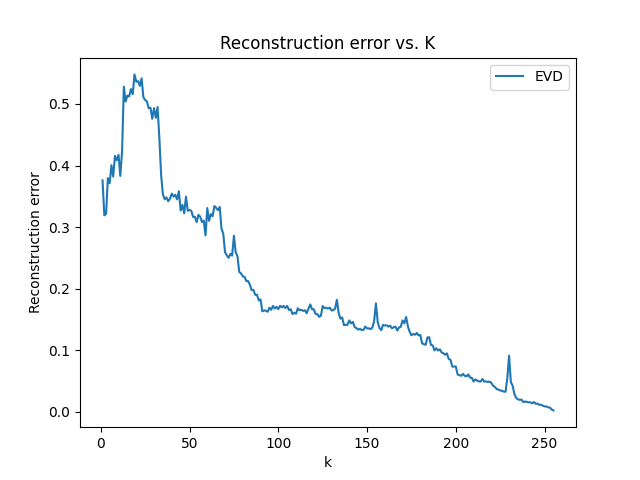
\includegraphics[scale= 0.5]{evd}
		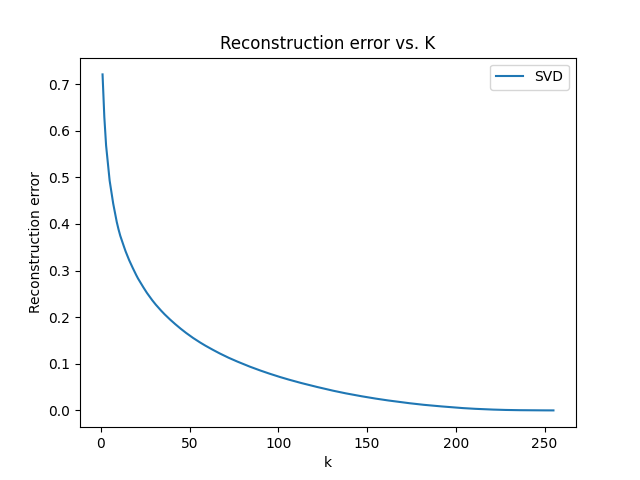
\includegraphics[scale= 0.5]{svd}
		\begin{center}
			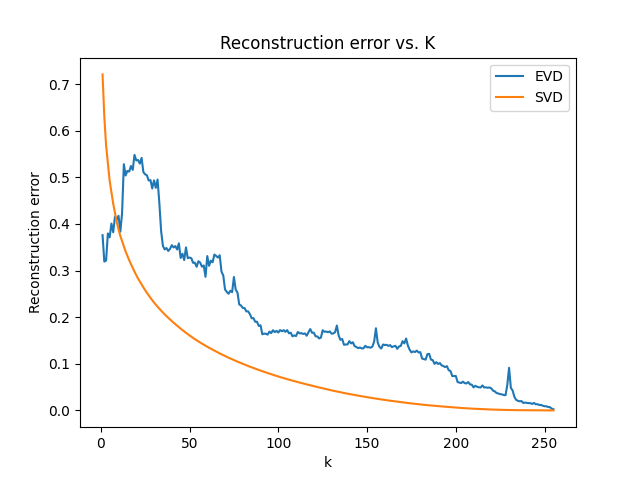
\includegraphics[scale= 0.5]{both}
		\end{center}
	\begin{large}
	\item \textbf{Inferences}
	\end{large}\\
		\begin{itemize}
		\item From the comparison of the error vs k graph of EVD and SVD we can infer that SVD is more reliable for compressing an image than EVD
		\item We can get most part of image with very less values in SVD
		\item For some values of k in EVD we get spike in error in reconstruction
		\end{itemize}
\end{enumerate}

\end{document}